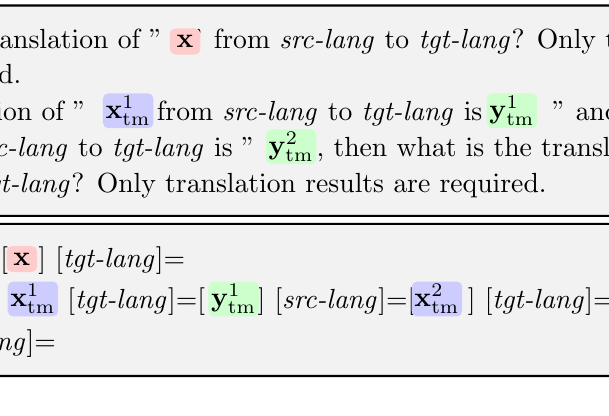
\begin{tikzpicture}
\useasboundingbox (-10em,-10em) rectangle (10em,3em);
\tikzstyle{modelnode} = [rectangle,draw=none,rounded corners=2pt,inner sep=2pt,minimum height=4.5em,minimum width=2em,font=\small,anchor=north,rotate=90]
% \node (a) at (0,0) {instruction-style template};
\node [draw=black,inner sep=0.4em,rounded corners=4pt,thick,fill=gray!10,minimum width=41.5em,minimum height=7.6em] (it) at (0,0){};
\node [draw=black,inner sep=0.4em,rounded corners=4pt,thick,fill=gray!10,minimum width=41.5em,minimum height=5.5em] (it_1) at ([xshift=0em,yshift=-3em]it.south){};
%%%%%%%%%%%%%%%%%%%%%%%%%%%%%
% What is the translation of "x" from src-lang to tgt-lang? Only translation results are required.
%%%%%%%%%%%%%%%%%%%%%%%%%%%%%%%
\node (b)[anchor=north,align=center] at ([xshift=-0.9em,yshift=-0.5em]it.north){$f(\cdot)$\hspace{0.87em}: What is the translation of "\hspace{1em}" from \textit{src-lang} to \textit{tgt-lang}? Only translation results};
\node (b_1) [anchor=south,align=center] at ([xshift=-12.1em,yshift=-1.2em]b.south){are required.};
\node (b_2) [anchor=south,align=center,fill=red!20,rounded corners=2pt,inner sep=2.5pt] at ([xshift=-3.41em,yshift=-1.33em]b.north){$\mathbf{x}$};
% \draw [rectangle,text width=5mm] at ([xshift=-16em,yshift=-3em]b.north){\small{N\\O\\I\\T\\C\\U\\R\\T\\S\\NI}};
\node [modelnode,align=center] (a) at ([xshift=-22em,yshift=-4em]it.north){\ttfamily{\textbf{INSTRUCTION}}};
%%%%%%%%%%%%%%%%%%%%%%%%%%%%
% If the translation of "X1" from English to Chinese is "Y1" and the translation of "X2" from English to Chinese is "Y2"···and the translation of "Xk" from English to Chinese is "Yk", then what is the translation of "X" from English to Chinese? Only translation results are required.
%%%%%%%%%%%%%%%%%%%%%%%%%%%%%%%
\node (c) [anchor=south,align=center] at([xshift=-0.62em,yshift=-4.8em]it.north){$f_{\mathrm{ref}}(\cdot)$: If the translation of "\hspace{1.7em}" from \textit{src-lang} to \textit{tgt-lang} is "\hspace{1.7em}" and the translation of};
\node(c1) [anchor=south,align=center,fill=blue!20,,rounded corners=2pt,inner sep=1pt] at ([xshift=-5.75em,yshift=-1.4em]c.north){$\mathbf{x}_{\mathrm{tm}}^{1}$};
\node(c1_1) [anchor=south,align=center,fill=green!20,,rounded corners=2pt,inner sep=1pt] at ([xshift=8.12em,yshift=-1.4em]c.north){$\mathbf{y}_{\mathrm{tm}}^{1}$};
\node (c1_1) [anchor=south,align=center] at ([xshift=1.49em,yshift=-1.25em]c.south){"\hspace{1.7em}" from \textit{src-lang} to \textit{tgt-lang} is "\hspace{1.7em}", then what is the translation of "\hspace{1em}" from};
\node (c1_2) [anchor=south,align=center] at ([xshift=-4.9em,yshift=-1.3em]c1_1.south){\textit{src-lang} to \textit{tgt-lang}? Only translation results are required.};
% \node (c1_3) [anchor=south,align=center] at ([xshift=-9.15em,yshift=-1.25em]c1_2.south){Only translation results are required.};
 %  \textit{src-lang} to \textit{tgt-lang}? Only translation results are required.
\node(c1_2) [anchor=south,align=center,fill=blue!20,,rounded corners=2pt,inner sep=1pt] at ([xshift=-13.73em,yshift=-2.7em]c.north){$\mathbf{x}_{\mathrm{tm}}^{2}$};
\node(c1_3) [anchor=south,align=center,fill=green!20,,rounded corners=2pt,inner sep=1pt] at ([xshift=0.14em,yshift=-2.7em]c.north){$\mathbf{y}_{\mathrm{tm}}^{2}$};
% \node(c1_4) [anchor=south,align=center,fill=blue!20,,rounded corners=2pt,inner sep=1pt] at ([xshift=12.75em,yshift=-2.7em]c.north){$\mathbf{x}_{\mathrm{tm}}^{k}$};
% \node(c1_5) [anchor=south,align=center,fill=green!20,,rounded corners=2pt,inner sep=1pt] at ([xshift=-8.21em,yshift=-4em]c.north){$\mathbf{y}_{\mathrm{tm}}^{k}$};
\node(c1_6) [anchor=south,align=center,fill=red!20,,rounded corners=2pt,inner sep=2.5pt] at ([xshift=14.9em,yshift=-2.65em]c.north){$\mathbf{x}$};
% \node (c_2) [anchor=south,align=center] at ([xshift=-7.7em,yshift=-1.25em]c_1.south){Only translation results are required.};
\node (d) [modelnode,align=center] at ([xshift=-4.5em,yshift=-6.7em]a.south){\ttfamily{\textbf{CODE}}};
\node (e) [anchor=south,align=center] at ([xshift=5.75em,yshift=0.6em]d.south){$f(\cdot)$\hspace{0.86em}: [\textit{src-lang}]=[\hspace{1.1em}] [\textit{tgt-lang}]=};
\node (e1) [anchor=south,align=center,fill=red!20,,rounded corners=2pt,inner sep=2.5pt] at ([xshift=1.46em,yshift=-1.3em]e.north) {$\mathbf{x}$};
\node (f) [anchor=south,align=center] at ([xshift=17.1em,yshift=-0.9em]d.south){$f_{\mathrm{ref}}(\cdot)$: [\textit{src-lang}]=[\hspace{1.9em}] [\textit{tgt-lang}]=[\hspace{1.9em}] [\textit{src-lang}]=[\hspace{1.9em}] [\textit{tgt-lang}]=[\hspace{1.9em}] [\textit{src-lang}]=};
\node (f) [anchor=south,align=center] at ([xshift=-12em,yshift=-1.5em]f.south){[\hspace{1.1em}] [\textit{tgt-lang}]=};
\node (f1) [anchor=south,align=center,fill=blue!20,rounded corners=2pt,inner sep=1pt] at ([xshift=2.51em,yshift=0.1em]f.north){$\mathbf{x}_{\mathrm{tm}}^{1}$};
\node (f2) [anchor=south,align=center,fill=green!20,rounded corners=2pt,inner sep=1pt] at ([xshift=9.76em,yshift=0.1em]f.north){$\mathbf{y}_{\mathrm{tm}}^{1}$};
\node (f3) [anchor=south,align=center,fill=blue!20,rounded corners=2pt,inner sep=1pt] at ([xshift=17.11em,yshift=0.1em]f.north){$\mathbf{x}_{\mathrm{tm}}^{2}$};
\node (f4) [anchor=south,align=center,fill=green!20,rounded corners=2pt,inner sep=1pt] at ([xshift=24.31em,yshift=0.1em]f.north){$\mathbf{y}_{\mathrm{tm}}^{2}$};
% \node (f5) [anchor=south,align=center,fill=blue!20,rounded corners=2pt,inner sep=1pt] at ([xshift=-7em,yshift=-1.5em]f.north){$\mathbf{x}_{\mathrm{tm}}^{k}$};
% \node (f6) [anchor=south,align=center,fill=green!20,rounded corners=2pt,inner sep=1pt] at ([xshift=0.28em,yshift=-1.5em]f.north){$\mathbf{y}_{\mathrm{tm}}^{k}$};
\node (f2) [anchor=south,align=center,fill=red!20,rounded corners=2pt,inner sep=2.5pt] at ([xshift=-2.35em,yshift=-1.26em]f.north){$\mathbf{x}$};
\end{tikzpicture} 